
	
	\noindent \section{Problem 1} 

Finding a good biochemical marker for fat intake is an important problem in cancer
							prevention research. The total cholesterol level or derivative measures such as HDL and
							LDL are normally used. However, it is well known that these measures are highly variable
							within an individual and, therefore, may not be reliable measures of fat intake. Many
							studies have shown that carnitine, a betaine derivative, C7H15NO3, may be useful as an
							alternative biochemical marker for fat intake. \\
							
							\vspace{0.2cm} 
	\noindent  	To investigate the effectiveness of carnitine as a biochemical marker for fat intake, a
							randomized experiment was conducted on 14 female monkeys. During an initial run-in
							period of 12 weeks all monkeys were put on a high, exclusively polyunsaturated, fat diet
							to stabilize their carnitine levels (data not included). After the run-in period, monkeys were randomized to
							two groups. Those monkeys randomized to group 1 received a low, exclusively polyunsaturated,
							fat diet, while those in group 2 continued on the same diet as in the run-in period.
							At week 10 after randomization, the polyunsaturated fat was replaced by saturated fat in
							both groups, with those in group 1 receiving a low saturated fat diet and those in group
							2 receiving a high saturated fat diet. Thus, in the current design, there are two levels of
							fat in the diet, high fat and low fat, and two types of fat, saturated and polyunsaturated. \\
				
							\vspace{0.2cm} 
	\noindent 	Weekly measurements of total plasma carnitine were obtained starting the week of randomization.
							Measurements at weeks 10 through 15 post randomization were not taken
							because that period was considered a “washout” period. In other words, measurements
							were made at weeks 1-9 and weeks 16-30. The goal of the current analysis is to investigate
							the relationship between fat and carnitine. \\
				
							\vspace{0.2cm} 
	\noindent  	The file \texttt{monkey.dat} contains the following variables:
							\begin{itemize}
								\item id: animal id number
								\item group: group number (1=low fat diet; 2=high fat diet)
								\item cartn0: total carnitine (nmol/ml) at randomization (baseline carnitine measure)
								\item cartn1: total carnitine (nmol/ml) 1 week after randomization \\
								 \vspace{0.2cm} ...
								\item cartn30: total carnitine (nmol/ml) 30 weeks after randomization
							\end{itemize}
				
				
				
							\begin{itemize}
							  \vspace{0.2cm} 
								\item[(A)] In no more than two pages and using no more than four supporting tables and figures, descriptively 
													 summarize the data. Comment on any aspect of the dataset that you
													 feel is relevant to the interpretation of the data. \vspace{0.2cm}

The dataset "monkey.dat" consist of 14 subjects with 30 measurement of total plasma carnitine for each subject. The subjects were divided into two groups and were given two types of fat on schedule with the group 1 receiving a low fat diet and the group 2 receiving a high fat diet. Total 25 the total carnitine levels (nmol/ml) were measured for individuals at weeks 1-9 and weeks 16-30. There are 5 missing values for the subjects 1, 3, 4, 10, and 11 at week 22. That is, the data is balanced but not complete.
We would like to transform the dataset from one subject one record format to long format for descriptive analysis. First, we would like to look at the spagetti plots of the carnitine trajectory over time for each group using panel plot (Figure $\ref{fig:describ1}$). 

\begin{figure}
    \centering
    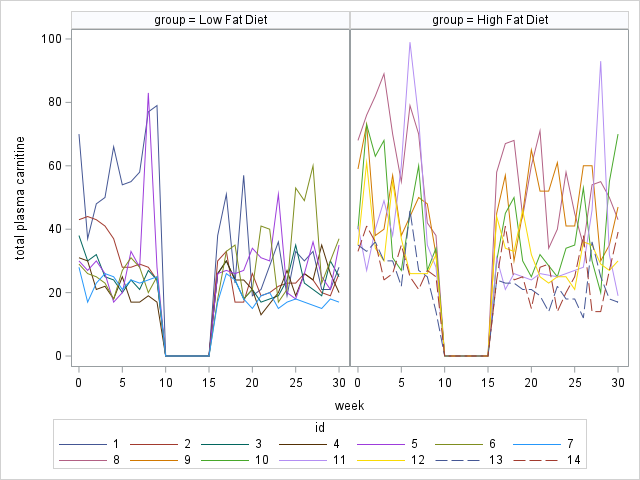
\includegraphics[scale=1]{HW4/img/desc1.png}
    \caption{Carnitine Trajectory}
\label{fig:describ1}
\end{figure}

Overall, we could see that the carnitine measurements are higher in group 2, which is high fat diet. And we could see a linear increasing trend between the carnite measurements and time in both groups. 

								\vspace{0.2cm}
								\item[(B)] It is of interest to explore the differences in total carnitine between the high and low
													 fat diets after adjusting for the baseline carnitine level. Answer this question using
													 the week 9 measurement as the outcome variable. In your report, be sure to do the following:
													 
												\begin{itemize}
													\vspace{0.2cm}
													\item[(i)] Develop an appropriate analysis plan. Write an explicit form for your model.
																		 State any assumptions needed for estimation, inference, and hypothesis testing.

If we only look at the difference at week 9 carnitine level, then we will do a cross section analysis. We will use the adjusted baseline change score by subtracting the baseline response from the week 9 measurement, and analyze the differences from baseline. 

The model is as below:

\begin{align*}
Z_{i} &=  \beta_{1}  +  \beta_2 I(group= 2) + \epsilon
\end{align*}

where $Z_{i}= Y_{ij} - Y_{i0}$ is the measurement change at week 9 than the baseline. 

The assumption of error term is $\epsilon \sim N(0, \sigma^2)$, which means that the errors are i.i.d (independent, identical) Gaussian distribution regardless of group. 

The hypothesis test are:
\begin{align*}
H_0: & \beta_2 = 0 \\
H_1: & \beta_2 \neq 0
\end{align*}

													\vspace{0.2cm}
												  \item[(ii)] Conduct the analysis and provide results.	This includes any diagnostic or sensitivity analyses
																			that you feel are appropriate.

The diagnostic analysis mainly focus on the influential and outlier points. For linear model, we could look at the scaled residual and Cook's distance.


													
													\vspace{0.2cm}
												  \item[(iii)] Provide a summary of your analysis results in language the investigator can understand. All tables 
																			 and figures included in the summary should be accompanied by sufficient exposition to help the 
																			 investigator understand the purpose of the table or figure. 		
											   \end{itemize}
								
								\vspace{0.2cm}
								\item[(C)] Conduct a repeated measures analysis using the first 9 weeks of measurements to study the effect of high 
													 versus low fat diets on total carnitine after adjusting for the baseline carnitine level. In your report, 
													 be sure to include the following:
							
													\begin{itemize}
													\vspace{0.2cm}
													\item[(i)] Develop an appropriate analysis plan. Write an explicit form for your model.
																		 Given the small sample size, discuss relevant assumptions and selection of method needed for estimation, inference, and hypothesis testing.

For repeated measures analysis with random effect model, the measurements within the same subject are correlated, and we assume the variance structure is compound symmetry considering small sample size. 

The model is as below:

\begin{align*}
Y_{ij}| b_i &= \beta_{01} I(group=1) + \beta_{02} I(group= 2) + \beta_{11} I(group=1) Y_{01}  + \beta_{12} I(group=2) Y_{02} + \beta_{21} I(group=1) Time_{j}  + \beta_{22} I(group=2) Time_{j} + b_{i} +  \epsilon_{ij}
\end{align*}

where $Y_{ij}$ is the measurement at week 9, and the assumption of error term is as below:
\begin{align*}
b_{i} & \sim N(0, \sigma_b^2) \\
 \epsilon_{ij} & = \begin{cases} 
 N(0_{n_i}, \sigma_1^2 I_{n_i}) & group = 1 \\
 N(0_{n_i}, \sigma_2^2 I_{n_i}) & group = 2 
\end{cases}
\end{align*}
Here we assume difference error structures for different groups, so the error term for subject $i$ is:
\begin{align*}
Var(Y_{ij}) & = \begin{cases} 
 \sigma_1^2 + \sigma_b^2 & \sigma_b^2 &.. & \sigma_b^2 \\
 \sigma_1^2 + \sigma_b^2 & \sigma_b^2 &.. & \sigma_b^2 \\
\end{cases}
\end{align*}

Both the subject effect and the measurement error are assume to be random, with mean zero, and with variances as above. In addition, it is assumed that $b_i$ and $\epsilon_{ij}$ are independent of one another. 
  
The hypothesis test are:
\begin{align*}
H_0: & \beta_{01} = \beta_{02} , \quad \text{and} \beta_{21} = \beta_{22} \\
H_1: & \beta_{01} \neq  \beta_{02}  , \quad \text{or}  \beta_{21} \neq \beta_{22} 
\end{align*}

For estimation and hypothesis tesing, REML method was used and the method developed by Kenward and Roger was used for the degree of freedom.
	
													\vspace{0.2cm}
												  \item[(ii)] Conduct the analysis and provide results.	This includes any diagnostic or sensitivity analyses
																			that you feel are appropriate.
													
													\vspace{0.2cm}
												  \item[(iii)] Provide a summary of your analysis results in language the investigator can understand. All tables 
																			 and figures included in the summary should be accompanied by sufficient exposition to help the 
																			 investigator understand the purpose of the table or figure. 		
											   \end{itemize}						
							
							
								\vspace{0.2cm}
								\item[(D)] Compare the analyses in parts (B) and (C). Which analysis is more appropriate for this data set? Justify your answer.							
							
								\vspace{0.2cm}
								\item[(E)] We are also interested in investigating whether there is an impact of ``switch-over'' from polyunsaturated fat 
													 to saturated fat on the carnitine levels and whether the impact is different for the high fat and low fat diets. 
													 To address these issues, perform an analysis using all available measurements. Baseline carnitine should be 
													 adjusted for in the analysis. In your report, be sure to include the following:
							
													\begin{itemize}
													\vspace{0.2cm}
													\item[(i)] Develop an appropriate analysis plan. Write an explicit form for your model.
																		 State any assumptions needed for estimation, inference, and hypothesis testing.
	
													\vspace{0.2cm}
												  \item[(ii)] Conduct the analysis and provide results.	This includes any diagnostic or sensitivity analyses
																			that you feel are appropriate.
													
													\vspace{0.2cm}
												  \item[(iii)] Provide a summary of your analysis results in language the investigator can understand. All tables 
																			 and figures included in the summary should be accompanied by sufficient exposition to help the 
																			 investigator understand the purpose of the table or figure. 		
											   \end{itemize}								

   \end{itemize}	
				
\newpage


	\noindent \textbf{Problem 2} -- Adults with intellectual and developmental disabilities (IDD) are living longer, and an
																	increasing number are now living and working in the community instead of residing in
																	institutions. Because of the increasing number of middle-aged and older persons with IDD,
																	there is growing concern about cardiovascular disease (CVD) in the IDD population. This
																	concern is due to a number of studies showing that conditions related to CVD may be
																	more prevalent in the IDD population and may affect persons with IDD at a younger age
																	than in the general population. \\
																	
																	\vspace{0.2cm}
																	UNC investigators plan to collect data on adults with mild to moderate IDD served
																	by compensatory education programs in North Carolina community colleges. In a pilot
																	study, they learned that IDD adults had HDL (``good'') cholesterol levels much lower
																	than those in the general population. They plan to conduct a study in 5 community
																	colleges to determine whether a walking for exercise intervention can be used to increase
																	HDL cholesterol levels among IDD adults. Within each community college, 100 adults
																	with IDD will be randomized to two groups, each with 50 adults: walking for exercise, or
																	placebo. Each subject will have HDL cholesterol measured at $t=0$ months (baseline), $t=6$ months,
																	and $t=12$ months. (Walking has been shown to be an effective way to increase
																	HDL cholesterol to healthy levels.) \\
																	
																	\vspace{0.2cm}
																	The investigators will fit the linear mixed effects model for subject $i$ in college $h$ at month
																	$t$:
																	\[
																			Y_{hit} = \beta_0 + \beta_1t + \beta_2 t x_{hi} + u_h + b_{hi} + \epsilon_{hit},
																	\]
																	where $\epsilon_{hit} \overset{iid}{\sim} \text{N}\left(0,\sigma^2_e\right)$ independent of 
																	$b_{hi} \overset{iid}{\sim} \text{N}\left(0,\sigma^2_b\right)$ independent of 
																	$u_{h} \overset{iid}{\sim} \text{N}\left(0,\sigma^2_h\right)$. The variable $x_{hi} = 1$
																	if the participant is randomized to the walking exercise group and $x_{hi} = 0$ if randomized
																	to placebo.
																	%
																	Integrating over the random effects, they expect that the marginal distribution of $Y_{hit}$ (mg/dL HDL cholesterol) 
																	in the control group would be approximately normally distributed with mean $50$ and variance $13^2$. They would like to 
																	know the minimum detectable effect of the walking program (measured by $\beta_2$) for a linear time trend  
																	assuming that $\beta_0$ = 50 and $\beta_1 = 0.01667$, using a 2-sided test with type I error 
																	rate of 5\% and power equal to 80\%. For the error structure, they assume that observations on the same adult should have 
																	correlation 0.60 regardless of their spacing in time and that observations on different adults at the same community college 
																	should have correlation 0.20. \\
																	
								\begin{itemize}
								\vspace{0.2cm} 
								\item[(A)] Clearly describe the steps you will take to calculate the minimum (absolute) detectable value of $\beta_2$ for the study above, providing all
								           important details regarding the simulation study performed. Give the values of the variance components implied by the information provided. 		


								\vspace{0.2cm} 
								\item[(B)] Provide the minimum detectable $\beta_2$ if the investigators carry out the study in 5 North Carolina community colleges, randomizing exactly
													 50 adults to placebo and 50 adults to the walking intervention within each community college. Assume that follow-up rates are 100\% (i.e., no missing data).


								\vspace{0.2cm} 
								\item[(C)] Investigators may gain additional financial support, which they could use to (i) double the number of community colleges from 5 to 10, keeping 100 adults in 
													 each, (ii) double the number of adults recruited within each community college, so retaining 5 colleges with 200 subjects each, or (iii) double the number of 
													 follow-up visits of the existing subjects (to approximately 0, 2.4, 4.8, 7.2, 9.6, and 12 months). Advise investigators regarding which approach is optimal 
													 (with respect to having the smallest detectable $\beta_2$ in absolute value) under the setup above. Provide statistical evidence to support your advice. Optimal
													 solutions will produce a graphic of the power function ($\beta_2$ on the x-axis, power and the y-axis).

								\vspace{0.2cm} 
								\item[(D)] Assuming the investigators use the setup in part (a), they wish to conduct a power calculation that accommodates missing data. Suppose that the missing data satisfy 
													 monotone dropout are otherwise generated as follows. Let $R_{hit}=1$ indicate that $Y_{hit}$ is missing (and hence all future measurements).
														\[
																 \text{logit}\left[\text{P}\left( R_{hit} = 1 \big|  \mathbf{Y}_{hi}\right)\right] = 3.95 - 0.09 \cdot Y_{hi,t-1},
														\]
													 for $t>0$ and that all participants have an observed value of $Y_{hit}$ at time $t=0$. Are the missing data MCAR, MAR, or NMAR in this case? Is it meaningful 
													 to consider the power of the test in this setting? Explain. If it is meaningful, what is the minimum detectable value of $\beta_2$?
													 \end{itemize}
							

